\setchapterimage[8.5cm]{outlook/lsst}
\setchapterpreamble[u]{\margintoc}
\chapter{Summary and Future Outlook}
\labch{summary}
\begin{fquote}[Ambrose Bierce][The Cynic's Dictionary][1906] FUTURE, n. That period of time in which our affairs prosper, our friends are true and our happiness is assured.  
\end{fquote}

This thesis has presented an archival search for correlations between TDEs and IceCube neutrinos, with no significant correlation reported. It has also presented the first strong evidence of a correlation between high-energy IceCube neutrino alerts and ZTF-detected TDEs. The former result suggests that TDEs do not contribute more than 39?\% of the neutrino flux, while the latter result suggests that they contribute at least 2?\%. These two results rely on different reconstructions, data selections and analysis frameworks. There is clearly a lot of space open to be probed by future studies.

Because of latency in IceCube data processing, the TDE-neutrino correlation analysis presented in Chapter \ref{ch:results} only considered TDEs discovered before 2018. In the subsequent three years, ZTF has substantially increased the number of well-characterised TDEs, with the overall sample size more than doubling. An updated IceCube correlation analysis using more recent data would be substantially more sensitive than the one presented here. Of particular interest would be a search for lower-energy neutrinos from AT2019dsg, offering the opportunity to perhaps distinguish between different neutrino emission scenarios introduced in Chapter \ref{ch:bran}.  

Such correlation become more powerful as new transients are detected by wide-field surveys. At optical wavelengths, the volume of transient discovery will increase by another order of magnitude with the advent of the \emph{Vera C. Rubin Observatory} \sidecite{lsst_19}, providing a comprehensive accounting of the dynamic sky to depth of >24 mag. Beyond optical, new and upcoming surveys include the \emph{UltraSat} at UV wavelengths \sidecite{ultrasat_14}, \emph{eROSITA} for X-rays \sidecite{erosita_21}, and \emph{CTA} for $\gamma$ rays \sidecite{cta_11}. Jointly, these surveys will provide a powerful baseline for transient multi-messenger studies.

In the near future, the seven-string \emph{IceCube Upgrade} will also be deployed \sidecite{ic_upgrade}. This dense in-fill array is primarily designed to extend IceCube's sensitivity to lower-energy (GeV) neutrinos, and will thus most directly impact studies of neutrino oscillations and low-energy transients. However, the IceCube Upgrade also includes extensive calibration hardware, and may thus have a large indirect impact on IceCube neutrino astronomy performance. Better modelling of uncertainties such as the ice properties may lead to substantially-revised reconstructions and angular error estimates, and thus reveal previously-obscured correlations in archival neutrino data.

\begin{figure}
	\centering 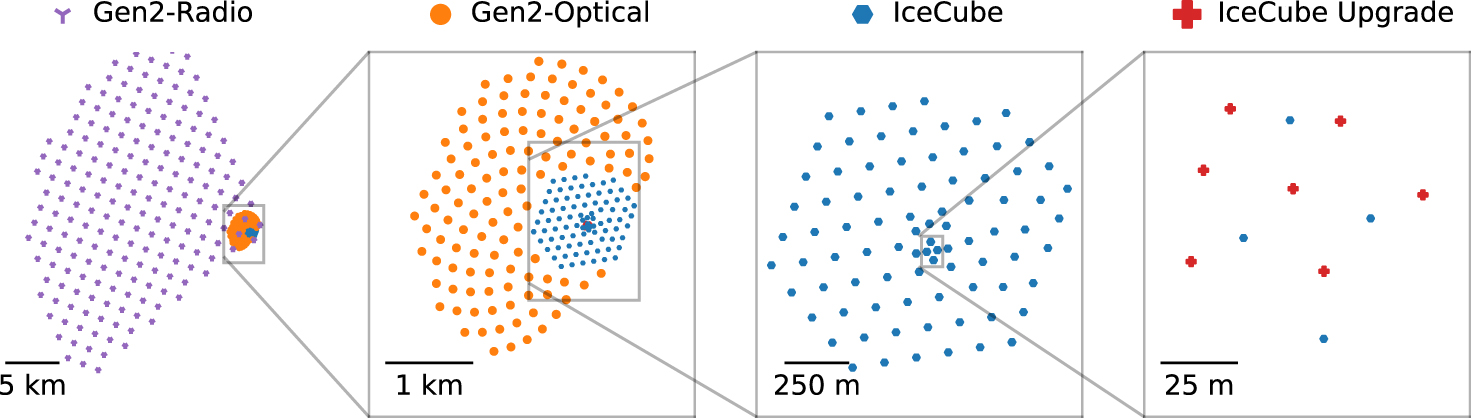
\includegraphics{outlook/ic_gen2_design}
	\caption{Layout of IceCube-Gen2 and the IceCube Upgrade in comparison to IceCube, from \cite{ic_gen2_21}.}
	\label{fig:gen2_layout}
\end{figure}

More significantly, the \emph{IceCube-Gen2} extension should begin deployment this decade \sidecite{ic_gen2_21}. This would expand the instrumented volume from the current 1 km$^{3}$ to a total of 7.9 km$^{3}$, yielding  a substantial increase in the rate of high-energy neutrino detections. However, due to cost constraints, the new volume would have a lower DOM density which will impact event reconstructions at lower energies. While the individual DOMs themselves are likely to be more effective multi-PMT detectors, IceCube-Gen2 will still represents a transition in energy range, with a median energy of 30 TeV rather than 10 TeV for IceCube. This transition is also relevant in terms of sensitivity, because the IceCube detector has operated primarily as a 4$\pi$ detector, or at least a $2 \pi$ one. However, for higher energies the impact of Earth absorption becomes more significant, so as seem in Figure \ref{fig:gen2_sens} the enhanced sensitivity of the detector at the horizon will become somewhat more pronounced. 

\begin{marginfigure}
	\centering 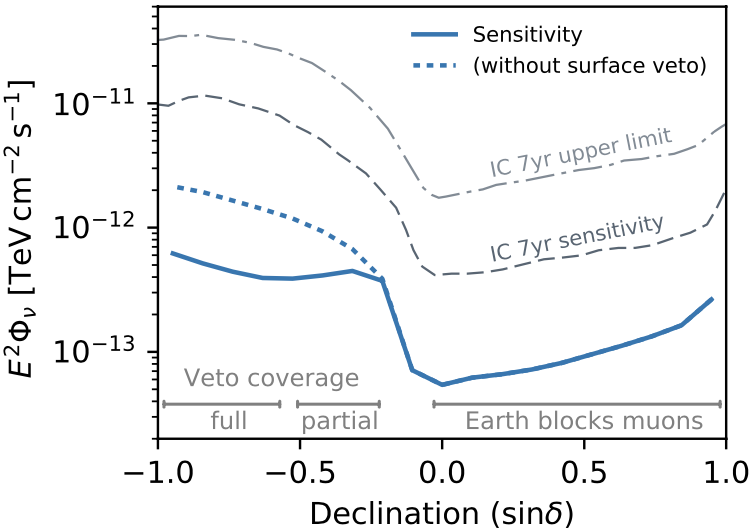
\includegraphics{outlook/gen2_sens}
	\caption{Sensitivity of IceCube-Gen2 (orange) in comparison to IceCube (blue), from \cite{gen2_icrc}. The dotted line shows the sensitivity without surface veto.} 
	\label{fig:gen2_sens}
\end{marginfigure}

A further radio-based extension is proposed to complement the DOM-based Gen2 component. The detection of radio-based air shower detection has been demonstrated by the Pierre Auger Observatory \sidecite{pao_radio_14}, and its use in ice was pioneered by the ARA and ARIANNA collaborations \sidecite{ara_12, arianna_14}. A pilot array for neutrino detection is currently being deployed in Greenland \sidecite{rnog_21}. Radio-based observatories are cheap, and given the possibility of single-station shower detection, an extremely sparse array can be deployed to substantially boost effective area. The proposed radio-based component for Gen2, with 200 stations across 500km$^{2}$, would significantly improve sensitivity at the higher energies beyond $\sim$10 PeV, and could additionally probe the cosmogenic neutrino flux produced by interactions of UHECRs and CMB photons \cite{ic_gen2_21}.

The AMANDA detector discovered atmospheric neutrinos, and served as a stepping stone to IceCube. IceCube, now in full operation for over a decade, successfully established neutrino astronomy with the discovery of he astrophysical neutrino flux, but has a characteristic signal-to-noise which has so far only proved sufficient to provide 3$\sigma$ hints of neutrino sources. With luck, IceCube-Gen2 could mark the transition of neutrino astronomy to a mature field, in which 5$\sigma$ discoveries become routine. At this point, focus will shift from finding sources to characterising them. Neutrino population studies, indeed neutrino tomography and spectroscopy, are powerful scientific tools that we are not yet capable of leveraging, but could in future teach us much about astrophysical objects. Further, a well-characterised flux of astrophysical neutrinos would also provide an ideal tool for testing particle physics at the very highest energies.

IceCube is not the only multi-messenger observatory that will be upgraded. During the upcoming fourth observing run (O4), LIGO and Virgo will again improve their sensitivity, and will be also joined by the new Kagra observatory. This will increase the precision with which nearby kilonovae can be localised, increasing the probability that a successor to GW170817 is found. In the future, this multi-messenger populations could be used for more competitive measurements of the Hubble constant, or precision tests of general relativity. 

When this thesis work was started in 2017, the only examples of multi-messenger sources were the sun and galactic supernova SN1987A. In just four short years, new extragalactic multi-messenger transient detections have now transformed both neutrino and gravitational-wave astronomy. In the future, it is inevitable that such detections will cease to be exceptional, instead become a routine technique of astronomy. 
